\begin{enumerate}
\item \textbf{Data Collection:} \\
% Jana's task:
To train the model, we decided to use the crowd sourced CREMA-D data \cite{cremad} set that is downloadable from kaggle.com under the Open Data Commons Attribution License (ODC-By). This license allows to copy, distribute and use the database, furthermore to produce works from the database and to modify, transform and build upon it \cite{odc-by}.

The data set consists of 7,442 audio clips with the following characteristics: 
\begin{itemize}
    \item 12 different sentences
    \item six different emotions: Anger, Disgust, Fear, Happy, Neutral, Sad
    \item four different emotion levels: Low, Medium, High, Unspecified
    \item number of actors: 91
    \begin{itemize}
        \item age: ranging from 20 to 74 years
        \item ethnicity: African American, Asian, Caucasian, Hispanic, Unspecified
    \end{itemize}
\end{itemize}



\item \textbf{Preprocessing for Training:} \\
% Jana's task:
To increase the number and variety of data samples and to ensure robustness of the system to non-trivial scenarios, we will perform data augmentation in the form of random pitch shifts and time stretch transformations. Here, the python libraries Audiomentations and Librosa are useful. Both libraries are open-source and available for free. 

Then, we will calculate spectrograms from the raw audio samples by running a Fast Fourier Transform (FFT) algorithm. Here, again Librosa comes in handy. The spectrograms can then be fed into the neural networks.  

\begin{figure}[h]
\centering

\includegraphics[width=0.9\textwidth]{images/ser-preprocessing.png}\\
\caption{Preprocessing for Training.}\label{fig:ser_preprocessing}
\end{figure}

%\item \textbf{Feature Extraction:} 
\item \textbf{Modeling:} As already presented in chapter \ref{chap:project-ideas}, we are goint to use two different approaches for \acrshort{ser}, as is displayed in figure \ref{fig:ser_modeling}.\\
% Jana's task:
\emph{1. Approach: phonological information}

For the first approach, we will create a \acrfull{crnn},  i.e. a sequential neural network with 1D convolutional layers. It will take the spectrograms as input and outputs the most likely emotion associated with the input. Here, the python library Keras can be used to easily build a neural network by adding desired layers to the model. Keras is open-source and available for free. 

\emph{2. Approach: semantic information}

For the second approach, a combination of two neural networks will be used. First, an \acrfull{asr} model transforms the spectrograms into a textual representation of the utterance. This can again be done with Keras as it additionally offers APIs to pre-trained ASR models like DeepSpeech, an open-source model by Mozilla.
Then, the obtained text is assigned to an emotion by a transformer-based neural network. Here, the python library Hugging Face can be used. It is free, open-source and offers pre-trained transformer models like BERT. 
Since the ASR model and the transformer model are already pre-trained on a large corpus of data and our application scenario is kept general instead of domain-specific, it is not strictly necessary to find additional datasets for training the ASR model and the transformer model ourselves. \\

\begin{figure}[h!]
\centering
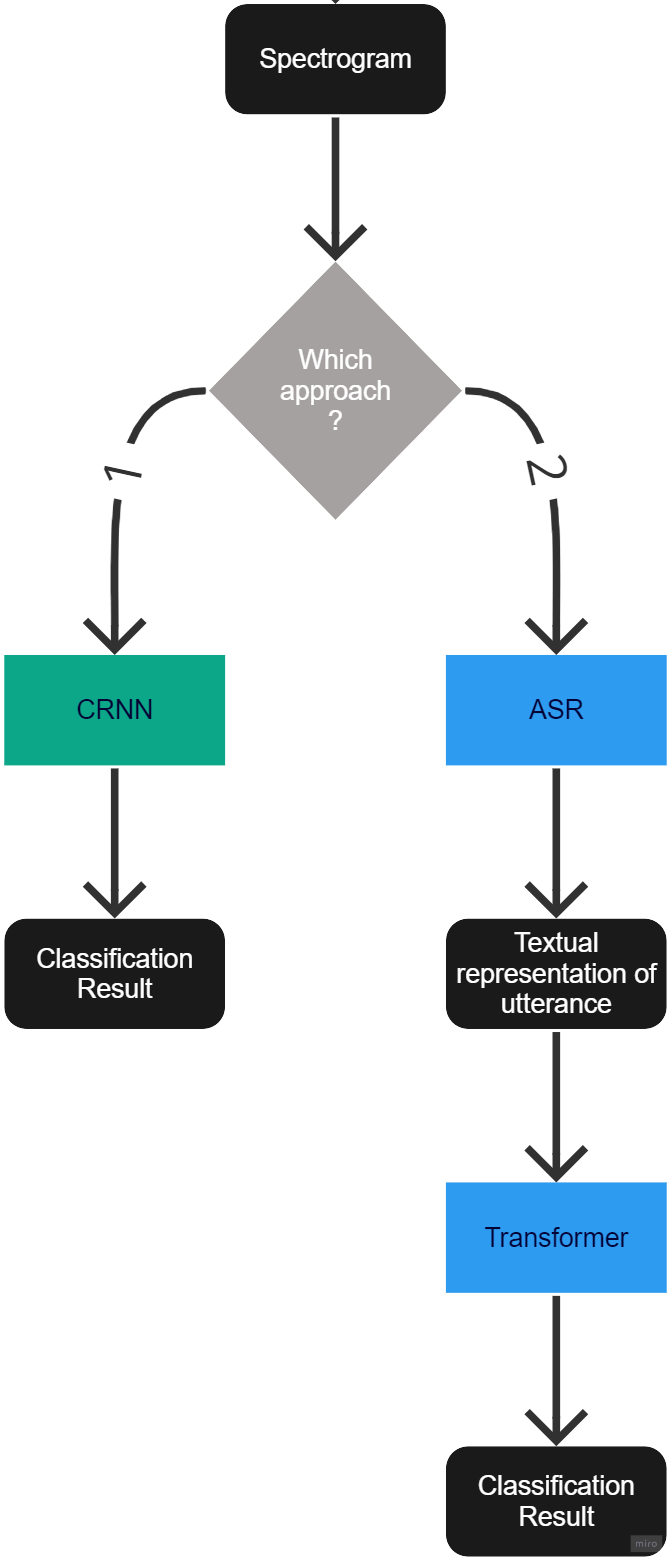
\includegraphics[scale=0.5]{images/SER_Modeling.png}\\
\caption{Modeling.}\label{fig:ser_modeling}
\end{figure}



\item \textbf{Model Evaluation:} \\
Test where we will run the model with a given input and compare its output with an expected output. The goal is to keep a track of the precision and loss of the model in training. The model must have a loss under a certain value and a precision above a certain value. During the development, we will also take advantage to unitary test for code coverage, these unitary tests will be needed to validate commit on the source control (GitHub in our case) of the project. Using this test will allow us to have an automated test pipeline that would be use for CI/CD. 

%Data splitting for Cross-Validation
%True positive (TP), True negatice (TN), False positive (FP), False negative (FN) when the model is not able to recognize any emotion.
%\begin{itemize}
%    \item Accuracy test,
%    By calculating how accurate is the model, using the following formula, $Accuracy = \frac{TP + TN}{N_{outputs}}$, we can test the success rate of the model.
%
%    \item Precision Test
%    Using the following formula, $Precision = \frac{TP}{TP + FP}$, we can test among the positive answers, the true positive rate.
%    
%    \item Sensitivity Test
%    $Sensitivity = \frac{TP}{TP + FN}$
%
%    \item Specificity Test
%    $Sensitivity = \frac{TN}{TN + FP}$
%    
%\end{itemize}

\color{black}
\item \textbf{System Development:} \\
% Jana's task
To test the speech emotion recognition in real-world scenarios, the trained neural networks will be embedded in a pipeline. 
The first step will be to record the users' utterances with a microphone. The continuous audio stream should then be cut every $x$ seconds to obtain the data samples. These will be preprocessed and fed into the neural networks. The results from both of the approaches will then be continuously published on the user interface. Here, the users indicate whether one or both of the classifications are correct and if not, what their actual emotion was. The user feedback will be stored along the respective audio sample and then used to retrain the models after the session. 
\color{blue}
%\item \textbf{System Evaluation:} including Comparison with Previous Studies: \\
% Ergi's task:
%The use of speech audio data in various applications has raised ethical considerations, particularly regarding the privacy and confidentiality of the participants in the dataset. Collecting audio data without the consent of the participants or disclosing the identity of the speakers can be a violation of privacy. Moreover, the use of audio data for purposes other than those that were originally intended can also result in ethical dilemmas. It is essential to ensure that the audio data collected is used only for legitimate purposes and that participants' personal information is kept confidential.
%\item \textbf{Limitations and Future Work:} \\
\end{enumerate}

%\section{Preliminary results and findings}
%\section{Implications of the results}